\documentclass[11pt]{article}

% ---------- Paquetes ----------
\usepackage[utf8]{inputenc}
\usepackage[T1]{fontenc}
\usepackage[spanish]{babel}
\usepackage{amsmath}
\usepackage[margin=2.5cm]{geometry}
\usepackage{graphicx}
\usepackage{booktabs}
\usepackage{hyperref}
\usepackage{fancyhdr}
\usepackage{titlesec}
\usepackage{enumitem}
\usepackage{caption}
\usepackage{float}
\usepackage{array}
\usepackage{placeins}

% ---------- Estilo de secciones (todo en negro) ----------
\titleformat{\section}
  {\normalfont\Large\bfseries}
  {\thesection.}{0.5em}{}
\titleformat{\subsection}
  {\normalfont\large\bfseries}
  {\thesubsection.}{0.5em}{}

% ---------- Encabezado/pie de página ----------
\pagestyle{fancy}
\fancyhf{}
\renewcommand{\headrulewidth}{0.4pt}
\fancyhead[L]{\small Proyecto 2 -- Análisis Exploratorio}
\fancyhead[R]{\small CGIAR Eyes on the Ground}
\fancyfoot[C]{\small\thepage}

% ---------- Hipervínculos (negro, sin color) ----------
\hypersetup{
    colorlinks=true,
    linkcolor=black,
    urlcolor=black,
    citecolor=black,
    pdftitle={Proyecto 2 - Análisis Exploratorio: CGIAR Eyes on the Ground},
    pdfauthor={Osman Emanuel de León García}
}

\setlength{\parskip}{0.6em}
\setlength{\parindent}{0pt}

\begin{document}

% =====================================================
% PORTADA
% =====================================================
\begin{titlepage}
\centering

\vspace*{1cm}

{\large\textsc{Universidad del Valle de Guatemala}}\\[0.3cm]
{\large Facultad de Ingeniería}\\[0.15cm]
{\normalsize Departamento de Ciencias de la Computación}\\[2.5cm]

\rule{0.8\textwidth}{0.5pt}\\[0.6cm]

{\Huge\bfseries Proyecto 2}\\[0.4cm]
{\Large\bfseries Análisis Exploratorio de Datos}\\[0.5cm]
{\large\itshape Reto 16 -- CGIAR Eyes on the Ground Challenge}\\[0.6cm]

\rule{0.8\textwidth}{0.5pt}\\[2cm]

{\normalsize Detección de daño por sequía en imágenes de cultivos\\
como base para la automatización de reclamos de seguro agrícola}\\[3cm]

{\large Osman Emanuel de León García}

\vfill

{\normalsize Curso de Data Science}\\
{\normalsize Septiembre de 2026}

\end{titlepage}

% =====================================================
% ÍNDICE
% =====================================================
\tableofcontents
\newpage

% =====================================================
% 1. INVESTIGACIÓN PREVIA
% =====================================================
\section{Investigación previa}

El seguro agrícola basado en imágenes (\textit{picture-based insurance}) es un modelo que usan aseguradoras como ACRE Africa, junto con instituciones como CGIAR, para verificar reclamos de pequeños agricultores sin tener que enviar a un perito a revisar cada parcela en persona. El agricultor toma una foto del cultivo con el celular y la envía como evidencia del estado del terreno \cite{ceballos2018,ceballos2019}. Estudios de campo en India muestran que este enfoque reduce el riesgo de base frente al seguro indexado por clima, y que expertos pueden identificar la mayoría de los casos de daño severo a partir de estas fotos, sin evidencia de riesgo moral o selección adversa por parte de los agricultores \cite{ceballos2021}.

El daño por sequía se puede identificar a simple vista por señales como marchitamiento y enrollamiento de las hojas, decoloración hacia tonos amarillentos o cafés, y plantas notablemente más pequeñas de lo esperado para su etapa de crecimiento. Esto lo diferencia de otros daños presentes en el dataset, como la inundación (plantas caídas o suelo anegado) o la deficiencia de nutrientes (decoloración más uniforme, sin el marchitamiento típico de la sequía). Este tipo de clasificación visual de daño en cultivos a partir de fotos de celular también se ha trabajado con visión artificial en otros contextos, como la detección de enfermedades de plantas mediante redes neuronales convolucionales \cite{mohanty2016}.

Hoy en día este proceso de verificación es manual: un evaluador revisa cada foto enviada y decide el tipo y severidad del daño para calcular el pago. Esto es lento y no escala bien cuando muchos agricultores presentan reclamos al mismo tiempo, por ejemplo después de un evento climático fuerte, lo que retrasa pagos que muchas veces se necesitan con urgencia. Por esta razón, CGIAR lanzó en 2023 un reto abierto de ciencia de datos en la plataforma Zindi para desarrollar modelos que ayuden a automatizar este proceso de verificación \cite{zindi2023,sti2023}.

% =====================================================
% 2. SITUACIÓN, PROBLEMA CIENTÍFICO Y OBJETIVOS
% =====================================================
\section{Situación problemática, problema científico y objetivos}

\subsection*{Situación problemática}
Los pequeños agricultores de Kenia que dependen de seguros agrícolas enfrentan demoras en sus pagos porque la verificación de daño por sequía a partir de fotos se hace de forma manual, lo cual no escala ante el volumen de reclamos y retrasa la compensación económica en momentos críticos.

\subsection*{Problema científico}
¿Qué patrones existen entre las imágenes de cultivos, sus metadatos (etapa de crecimiento, temporada) y el tipo o severidad del daño reportado, que sirvan de base para automatizar la clasificación de daño por sequía en el proceso de verificación de reclamos?

\subsection*{Objetivos}

\textbf{Objetivo general:}
\begin{itemize}[leftmargin=1.2cm]
    \item Caracterizar el dataset de imágenes y metadatos de CGIAR Eyes on the Ground para identificar qué distingue al daño por sequía de otros tipos de daño y de los cultivos sanos.
\end{itemize}

\textbf{Objetivos específicos:}
\begin{enumerate}[leftmargin=1.2cm]
    \item Cuantificar la distribución y severidad del daño por sequía (\texttt{extent}) y ver cómo varía entre temporadas agrícolas y etapas de crecimiento.
    \item Determinar si la composición de tipos de daño cambia entre las cuatro temporadas registradas (LR2020, LR2021, SR2020, SR2021).
\end{enumerate}

% =====================================================
% 3. DESCRIPCIÓN DE LOS DATOS
% =====================================================
\section{Descripción de los datos}

El dataset de entrenamiento (\texttt{Train.csv}) tiene 26{,}068 filas y 6 columnas: \texttt{ID} y \texttt{filename} como identificadores, \texttt{growth\_stage} y \texttt{damage} como variables categóricas, \texttt{extent} como variable numérica (0-100\%), y \texttt{season} como variable temporal. El conjunto de prueba (\texttt{Test.csv}) tiene 8{,}663 filas con las mismas columnas, salvo \texttt{extent}, que es la variable que se pedía predecir en la competencia original.

\begin{table}[htbp]
\centering
\caption{Descripción de las variables del dataset}
\begin{tabular}{@{}p{2.7cm}p{3cm}p{8cm}@{}}
\toprule
\textbf{Variable} & \textbf{Tipo} & \textbf{Descripción} \\
\midrule
\texttt{ID} & Identificador & Identificador único del registro \\
\texttt{filename} & Identificador & Nombre del archivo de imagen asociado \\
\texttt{growth\_stage} & Categórica & Etapa de crecimiento del cultivo (Siembra, Vegetativo, Floración, Madurez) \\
\texttt{damage} & Categórica & Tipo de daño observado (8 categorías: Bueno, Sequía, Maleza, Deficiencia de nutrientes, Plaga, Enfermedad, Viento, Inundación) \\
\texttt{extent} & Numérica & Porcentaje de severidad del daño (0-100\%), solo distinto de 0 cuando \texttt{damage} es Sequía \\
\texttt{season} & Categórica & Temporada agrícola de la observación (LR2020, LR2021, SR2020, SR2021) \\
\bottomrule
\end{tabular}
\end{table}

No se encontraron valores nulos en ninguna columna. La variable \texttt{damage} está bastante desbalanceada: ``Bueno'' (44.6\%) y ``Maleza'' (35.4\%) concentran la mayoría de los casos, ``Sequía'' es el 17.3\% (4{,}516 casos), y el resto de categorías (Enfermedad, Inundación, Deficiencia de nutrientes, Plaga, Viento) suman entre todas menos del 3\%. La variable \texttt{growth\_stage} está más repartida: Vegetativo (38.4\%), Madurez (25.6\%), Floración (23.6\%) y Siembra (12.4\%).

% =====================================================
% 4. LIMPIEZA Y PREPROCESAMIENTO
% =====================================================
\section{Limpieza y preprocesamiento}

Como no hubo valores nulos en \texttt{Train.csv}, no fue necesario imputar nada. Sí se encontró que la variable \texttt{extent} solo tiene valores distintos de cero cuando \texttt{damage} es ``Sequía''; en las otras siete categorías siempre vale 0. Esto no es un dato faltante, sino una decisión de cómo se armó el dataset: la severidad porcentual solo se documentó para el daño de interés principal de la competencia. Por eso, el análisis cuantitativo de la sección 5 se hizo filtrando únicamente los registros de sequía.

Para la parte visual, como las imágenes vienen en archivos comprimidos grandes (\texttt{train.zip} de casi 6.5GB y \texttt{test.zip} de casi 2.2GB, alojados en Google Drive), se decidió no descomprimir el zip completo. En vez de eso, se armó una función en Python que descarga el zip una sola vez (si no existe ya localmente) y extrae solo una muestra balanceada de imágenes por cada tipo de daño, suficiente para el análisis visual sin tener que guardar ni esperar la descarga del dataset completo.

% =====================================================
% 5. EDA CUANTITATIVO
% =====================================================
\section{Análisis exploratorio cuantitativo: severidad del daño por sequía}

La severidad de sequía (\texttt{extent}) tiene una media de 40.96\% y mediana de 40\%, con bastante dispersión (desviación estándar de 24.75) y valores en todo el rango posible (0-100\%). La frecuencia baja poco a poco hacia los valores más altos: los casos de severidad 80-100\% son los menos comunes dentro del grupo de sequía.

\begin{figure}[htbp]
\centering
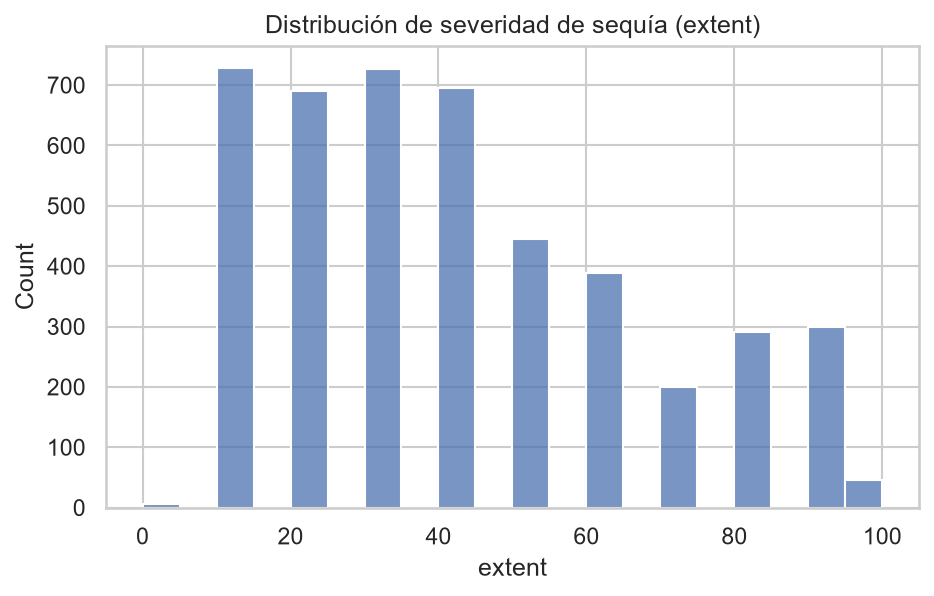
\includegraphics[width=0.62\textwidth]{figuras/hist_extent_sequia.png}
\caption{Distribución de la severidad de sequía (\texttt{extent})}
\end{figure}

No salieron valores atípicos a nivel global usando el criterio de rango intercuartílico (IQR): con $Q_1=20$ y $Q_3=60$, el IQR (40) es tan amplio que los límites de Tukey ($1.5 \times \text{IQR}$) quedan fuera del rango posible de la variable ($-40$ y $120$). Esto no es un error, simplemente refleja que la dispersión alta es normal en esta variable, no que haya valores raros.

Al ver los datos por temporada aparece el hallazgo más interesante de esta sección: mientras que la frecuencia de sequía se mantiene bastante estable entre temporadas (ver sección 6), la severidad sí cambia harto. La temporada SR2020 tiene la severidad promedio más alta (53.5\%), casi el doble que LR2021, la más baja (34.5\%).

\begin{figure}[htbp]
\centering
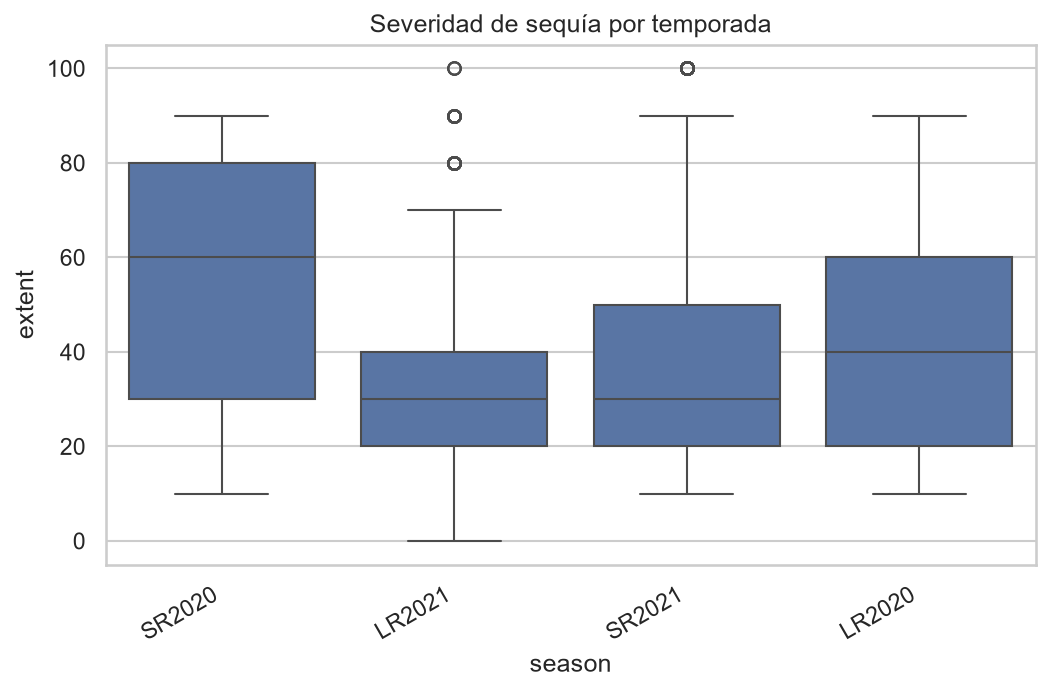
\includegraphics[width=0.62\textwidth]{figuras/box_extent_season.png}
\caption{Severidad de sequía por temporada}
\end{figure}

\begin{table}[htbp]
\centering
\caption{Estadística descriptiva de \texttt{extent} por temporada (solo \texttt{damage}=Sequía)}
\begin{tabular}{@{}lrrrr@{}}
\toprule
\textbf{Temporada} & \textbf{Media} & \textbf{Mediana} & \textbf{Desv. Est.} & \textbf{n} \\
\midrule
SR2020 & 53.5 & 60 & 28.8 & 1{,}146 \\
LR2020 & 43.1 & 40 & 24.9 & 391 \\
SR2021 & 37.1 & 30 & 23.1 & 1{,}566 \\
LR2021 & 34.5 & 30 & 18.2 & 1{,}413 \\
\bottomrule
\end{tabular}
\end{table}

Esto muestra que la frecuencia de sequía no dice mucho sobre qué tan fuerte es: SR2020 no solo tuvo casos de sequía, sino que en promedio fueron bastante más severos que en las demás temporadas.

Por etapa de crecimiento, Madurez tiene la severidad promedio más alta (43.35\%) y Floración la más baja (33.29\%) -- algo que llama la atención, porque uno esperaría que floración fuera de las etapas más vulnerables.

\begin{figure}[htbp]
\centering
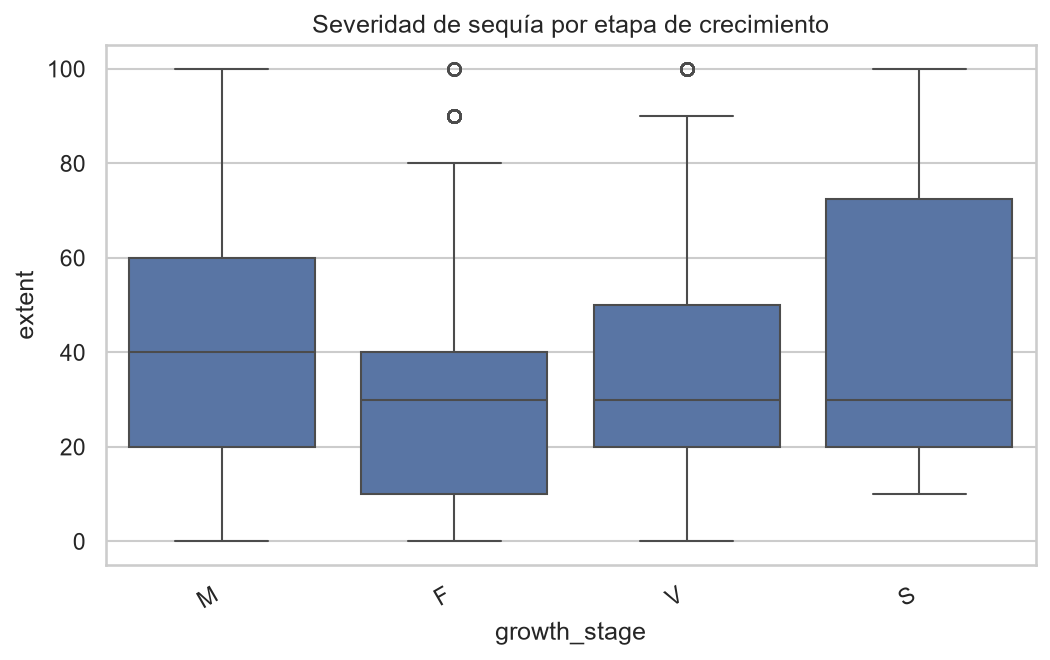
\includegraphics[width=0.62\textwidth]{figuras/box_extent_growth_stage.png}
\caption{Severidad de sequía por etapa de crecimiento}
\end{figure}

Aunque no hay outliers a nivel global, sí aparecen dentro de algunos subgrupos: en LR2021 (donde el IQR más angosto da un límite superior de 70) los valores de 80-100\% salen como atípicos, y pasa algo parecido en Floración (límite superior de 85). Esto muestra que lo que cuenta como valor ``extremo'' depende del contexto: valores comunes en SR2020 resultan raros en LR2021 o en Floración.

% =====================================================
% 6. EDA CATEGÓRICO Y VISUAL
% =====================================================
\section{Análisis exploratorio categórico y visual}

En general, ``Bueno'' es la categoría más común (44.6\%, 11{,}623 casos), seguida de ``Maleza'' (35.4\%, 9{,}238) y ``Sequía'' (17.3\%, 4{,}516); el resto de categorías juntas no llega al 3\% del total.

\begin{figure}[htbp]
\centering
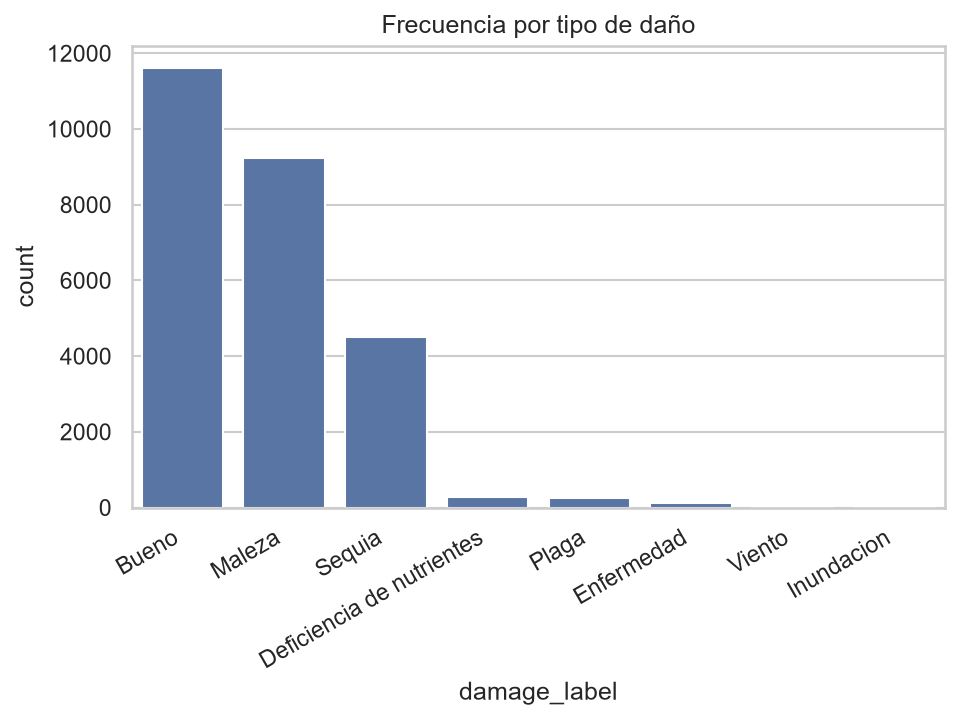
\includegraphics[width=0.58\textwidth]{figuras/barras_damage.png}
\caption{Frecuencia por tipo de daño}
\end{figure}

\begin{figure}[htbp]
\centering
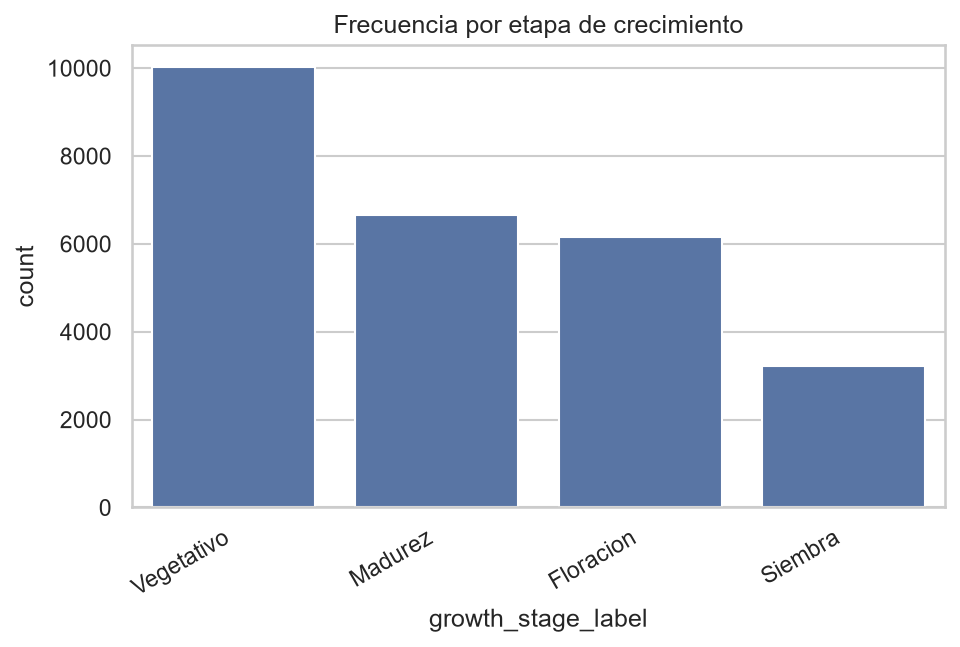
\includegraphics[width=0.58\textwidth]{figuras/barras_growth_stage.png}
\caption{Frecuencia por etapa de crecimiento}
\end{figure}

Al ver la frecuencia de sequía por temporada, se nota que se mantiene bastante estable: LR2020 (19.2\%), LR2021 (17.8\%), SR2020 (18.6\%) y SR2021 (15.8\%). En cambio, ``Bueno'' y ``Maleza'' son las que más cambian entre temporadas, lo que sugiere que otros factores -- no la sequía -- explican esas variaciones.

\begin{figure}[htbp]
\centering
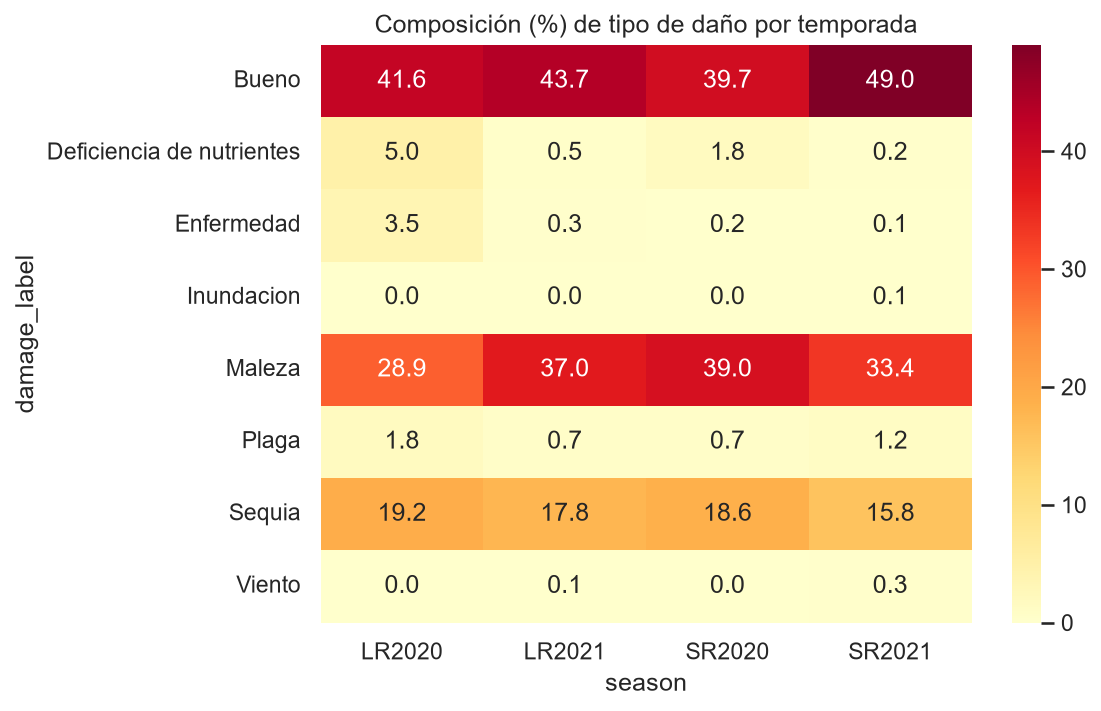
\includegraphics[width=0.62\textwidth]{figuras/heatmap_damage_season.png}
\caption{Composición porcentual de tipo de daño por temporada}
\end{figure}

El cruce entre daño y etapa de crecimiento es el hallazgo más importante de esta sección. Viendo qué porcentaje de cada etapa es sequía, se nota una progresión clara conforme el cultivo avanza en su ciclo:

\begin{table}[htbp]
\centering
\caption{Porcentaje de sequía dentro de cada etapa de crecimiento}
\begin{tabular}{@{}lrr@{}}
\toprule
\textbf{Etapa} & \textbf{\% de sequía dentro de la etapa} & \textbf{\% del total de sequía} \\
\midrule
Madurez & 48.6\% & 71.7\% \\
Floración & 13.9\% & 18.9\% \\
Vegetativo & 4.1\% & 9.0\% \\
Siembra & 0.6\% & 0.4\% \\
\bottomrule
\end{tabular}
\end{table}

Casi 7 de cada 10 registros de sequía del dataset ocurren en la etapa de Madurez, y casi la mitad de todas las observaciones de esa etapa son sequía. Esto se conecta directo con lo visto en la sección anterior: Madurez no solo es la etapa donde más ocurre la sequía, sino también donde es más severa en promedio. Las dos señales apuntan en la misma dirección: Madurez parece ser el momento del ciclo del cultivo con más riesgo de sequía.

Para respaldar esto con un número, se calculó Cramér's V entre pares de variables categóricas, que es una medida de asociación pensada justamente para este tipo de variable (a diferencia de la correlación de Pearson, que solo aplica a variables numéricas). Entre \texttt{damage} y \texttt{season} da 0.120, una asociación débil; entre \texttt{damage} y \texttt{growth\_stage} da 0.324, moderada y casi el triple que la anterior. Ambos resultados salen estadísticamente significativos ($p < 0{,}001$), pero lo que importa acá es la magnitud: confirma, con un valor concreto, que la etapa de crecimiento explica bastante más el tipo de daño que la temporada en la que se tomó la foto.

Por último, revisando una muestra balanceada de imágenes por clase, se nota una diferencia visual clara: las fotos de sequía tienen tonos café y amarillentos con plantas marchitas, mientras que ``Bueno'' y ``Maleza'' se ven más verdes y parejas. Sin embargo, hay bastante variedad en el ángulo, distancia y encuadre de las fotos dentro de una misma clase -- algunas son tomas de detalle del cultivo, otras del terreno completo -- lo que indica que las fotos no se tomaron de forma estandarizada, y eso podría meter ruido si más adelante se quisiera entrenar un modelo de clasificación basado solo en imagen.

% =====================================================
% 7. HALLAZGOS Y CONCLUSIONES
% =====================================================
\section{Hallazgos y conclusiones}

El análisis confirma que la sequía ocurre con una frecuencia bastante estable entre temporadas (16-19\% de los casos), pero su severidad varía harto: SR2020 tuvo la sequía más fuerte (media 53.5\%) y LR2021 la más leve (34.5\%). Esto responde al primer objetivo específico: la severidad del daño sí cambia entre temporadas, aunque su frecuencia no lo refleje.

El hallazgo más fuerte de todo el análisis es la relación entre sequía y etapa de crecimiento. La etapa de Madurez concentra el 71.7\% de todos los casos de sequía, y dentro de esa etapa casi la mitad de las observaciones (48.6\%) son sequía. Además, Madurez es también la etapa con mayor severidad promedio (43.35\%), mientras que Floración tiene tanto la menor frecuencia (13.9\%) como la menor severidad (33.29\%). Que frecuencia y severidad apunten en la misma dirección sugiere que el riesgo real de sequía se concentra en la etapa de madurez del cultivo, lo que responde al segundo objetivo específico.

Visualmente las clases sí se distinguen entre sí (tonos café/amarillentos y plantas marchitas en sequía, frente a un verde más uniforme en Bueno y Maleza), aunque la falta de estandarización en el ángulo y encuadre de las fotos es una limitación a tener en cuenta si más adelante se pensara en un modelo de clasificación por imagen.

Otra limitación es el desbalance de clases: ``Bueno'' y ``Maleza'' concentran cerca del 80\% de los datos, mientras que categorías como Inundación o Viento tienen menos de 40 casos cada una. Esto no afecta el análisis exploratorio en sí, pero sería un problema a resolver (por ejemplo con sobremuestreo o pesos de clase) si se entrenara un modelo de clasificación con estos datos más adelante.

En cuanto al problema científico planteado, los patrones encontrados -- sobre todo la fuerte relación entre madurez del cultivo y daño por sequía, tanto en frecuencia como en severidad -- dan una base razonable para pensar en automatizar la verificación de reclamos de seguro agrícola. Priorizar la revisión de fotos tomadas en etapa de madurez podría ser un buen punto de partida para un futuro sistema de clasificación automática, que ayude a reducir los tiempos de respuesta ante reclamos de agricultores afectados por sequía.

% =====================================================
% REFERENCIAS
% =====================================================
\newpage
\addcontentsline{toc}{section}{Referencias}
\begin{thebibliography}{9}

\bibitem{zindi2023}
Zindi. (2023). \textit{CGIAR Eyes on the Ground Challenge}. Recuperado de \url{https://zindi.africa/competitions/cgiar-eyes-on-the-ground-challenge}

\bibitem{sti2023}
FAO Science, Technology and Innovation Portal. (2023). \textit{``Eyes on the Ground Challenge'': A competitive online crowdsourcing program for developing machine learning models to analyze smartphone crop images for enhanced crop insurance solutions}. Recuperado de \url{https://sti-portal.fao.org/innovations/eyes-ground-challenge-competitive-online-crowdsourcing-program-developing-machine}

\bibitem{ceballos2018}
Ceballos, F., Kramer, B., \& Robles, M. (2018). \textit{The Feasibility of Picture-Based Insurance (PBI): Smartphone Pictures for Affordable Crop Insurance} (IFPRI Discussion Paper 1788). International Food Policy Research Institute.

\bibitem{ceballos2019}
Ceballos, F., \& Kramer, B. (2019). \textit{From Index to Indemnity Insurance Using Digital Technology: Demand for Picture-Based Crop Insurance} (IFPRI Discussion Paper 1890). International Food Policy Research Institute. Recuperado de \url{https://hdl.handle.net/10568/147049}

\bibitem{ceballos2021}
Ceballos, F., \& Kramer, B. (2021). \textit{The Role of Asymmetric Information in Multi-Peril Picture-Based Crop Insurance: Field Experiments in India} (IFPRI Discussion Paper 2088). International Food Policy Research Institute. \url{https://doi.org/10.2499/p15738coll2.134941}

\bibitem{mohanty2016}
Mohanty, S. P., Hughes, D. P., \& Salathé, M. (2016). Using deep learning for image-based plant disease detection. \textit{Frontiers in Plant Science}, 7, 1419. \url{https://doi.org/10.3389/fpls.2016.01419}

\end{thebibliography}

\end{document}
